\documentclass{article} % For LaTeX2e
\usepackage{nips12submit_e,times}
\usepackage{graphicx}
\usepackage{algorithmic}
\usepackage[ruled,vlined]{algorithm2e}
\usepackage{dsfont}
%\documentstyle[nips12submit_09,times,art10]{article} % For LaTeX 2.09
%\DeclareMathOperator{\argmax}{argmax}
%\DeclareMathOperator*{\argmin}{argmin}
%\DeclareMathOperator*{\Corr}{Corr}
\renewcommand{\vec}[1]{\mathbf{#1}}
\newcommand{\R}{\ensuremath{\mathds{R}}}
\usepackage{hyperref}
\title{Predicting political party affiliation from text}


\author{
Felix Bie\ss{}mann\thanks{\texttt{felix.biessmann@gmail.com}}
\And
Daniel Kirsch\thanks{\texttt{mail@danielkirs.ch}}
}
% The \author macro works with any number of authors. There are two commands
% used to separate the names and addresses of multiple authors: \And and \AND.
%
% Using \And between authors leaves it to \LaTeX{} to determine where to break
% the lines. Using \AND forces a linebreak at that point. So, if \LaTeX{}
% puts 3 of 4 authors names on the first line, and the last on the second
% line, try using \AND instead of \And before the third author name.

\newcommand{\fix}{\marginpar{FIX}}
\newcommand{\new}{\marginpar{NEW}}

\nipsfinalcopy % Uncomment for camera-ready version

\begin{document}


\maketitle

\begin{abstract}
Political parties are typically characterized by the opinions they propagate over some period of time. These political views are subject of the debates in political parliaments. We used the text of speeches and discussions in the German parliament to train a classifier that predicts the political party affiliation based on standard text features. We evaluate the classifier on parliament speeches and party manifestos. Besides the affiliation to a particular party we also investigate how well texts from members of the government can be distinguished from texts from members of the opposition. Moreover we analyse whether the texts contain words associated with positive or negative emotional polarity. Results indicate that automatic classification of political affiliation is possible with well above chance accuracy. Not surprisingly, our sentiment analysis shows political power correlates with the sentiment of a political speech: speeches are more positive when a party is in power and more negative when the text is from a member of the opposition. While some of these results are trivial findings, we also show how to use the models learned from parliament speeches to analyse texts for which the party affiliation is not clear, such as news articles or texts from lobby groups. 
\end{abstract}

\section{Introduction}

%During the last decades the methods used by governments to influence how other people think about their political decisions have changed. As most governments are subject to control by some form of democracy, they require the public opinion to be on their side. Which in turn requires to make customers of media products susceptible to the political views 
%Political views are largely influenced by content consumed mostly in text form. As most conflicts and problems reported on in media are too difficult 

In order to obtain an unbiased view on what is happening it is helpful to consider opinions from all parts of the political spectrum. This requires having a means of categorizing content to political parties. While it is trivial to attribute content to a political party if the speaker is known, this becomes much more difficult when we are given only the content in text form. 

We here propose a method for automatically associating content to political parties. Our approach learns a model that takes standard text features from speeches held in parliament discussions and the corresponding party as label. In this manuscript we provide some evidence using texts from the german parliament (Bundestag) \cite{plenarprotokolle} that automatic association of texts to political parties is possible with well above chance accuracy. 

As generalization performance of such an automatized system for political party prediction is difficult to measure, we also compare how well the learned models perform on the manifestos which the parties released before this governmental period \cite{linke_parteiprogramm, gruene_parteiprogramm,spd_parteiprogramm, cdu_parteiprogramm}. In order to interpret the features used by the model we also look at the correlations between the text features used by the model and the party label. We conjecture that this approach can yield some insights as to which discriminative features can be used by laymen to tell the political affiliation from texts that do not have clear party affiliations. 

Besides looking only at associations of text features and party membership we also looked at a slightly simpler problem, discriminating texts from members of the government and members of the opposition. In this simpler setting we were able to obtain accuracies on held-out data of above 0.85, which appears to be almost usable in practical applications. 

Finally we performed analyses that can be used to investigate whether the text of what a member of a given party said contains rather positive or negative sentiment. We find a strong correlation between political power, measured in seats in the parliament, and positive sentiment, meaning the more political power a party has, the more affirmative their speeches and the less power a party has, the more negative the content of their speeches become. Although this finding might seem somewhat trivial, it is as far as we know the first quantitative evaluation of this phenomenon on german politicians. 

\section{Methods}

In the following we list the steps we performed in order to learn a model that automatically attributes texts to parties. While not all of the experiments we tried are listed below, we made the code available on GitHub \cite{linksrechts_code}. The code should allow to download all data sources and run all experiments performed in this study. For more lightweight testing of the presented results we also provide a demo web site on which the model can be tested with plain text files or links to webpages containing the to-be-categorized text \cite{linksrechts}. 

\subsection{Data Collection}\label{sec:collection}
We extracted the texts from the official webpage of the German parliament \cite{plenarprotokolle}. The texts were split using regular expressions and party labels were extracted from the texts. The number of speeches for each political party is listed in \autoref{tab:results_four_classes}. 

Next to the parliament speeches we also extracted the text from the programs of each party for this legislative period \cite{linke_parteiprogramm, gruene_parteiprogramm,spd_parteiprogramm, cdu_parteiprogramm} and applied exactly the same preprocessing to these texts that we applied to the parliament speeches. Texts were split according to chapters in the respective texts, which resulted in an asymmetric number of data points per party, see also \autoref{tab:results_four_classes}.


\subsection{Data Cleaning}\label{sec:cleaning}
Prior to vectorization of the text data, we spent some efforts on cleaning the texts from noise-words. We did so to avoid biasing our classifier towards using words that are helpful for classifying parliament speeches but do not carry information about the actual target, political orientation\footnote{A classical example from computer vision of such kind of overfitting with machine learning methods was the winning approach of a 'tank-detection' challenge. On all images in the training set, the tank was depicted on a green field in front of blue sky, the negative examples did not feature this surrounding, so the classifier learned to detect green fields and blue sky and could perfectly detect tanks in this biased data set}. We first removed stopwords from the text, using a stopword list \cite{stopwords} and additional stopwords common to parliament speeches. Another option we considered for cleaning the text was to include all names of members of the parliament in the stopword list. Of course also the names of the parties themselves were removed from the text. Moreover we removed numbers and non-word symbols from the text. Finally we also removed sections from the texts that were not part of a speech and parts in the speeches that were short interruptions (applaus or critical remarks from other members of the parliament). As we did not have clear ideas what of these procedures was actually helpful for improving generalization performance, we optimized the cleaning procedure by including all options of the cleaning pipeline into the hyperparameter optimization, see \autoref{sec:crossvalidation}. 

\subsection{Bag-of-Words Vectorization}\label{sec:bow-vectorization}
Strings of teach speech are extracted using a bag-of-word vectorizer as implemented in scikit-learn \cite{scikit-learn}. The general idea of bag-of-words vectors is to simply count occurences of words (or word sequences, also called {\em n-grams}) for each data point (usually documents, here parliament speeches). So the text of each speech is transformed into a vector $\vec{x}\in\mathds{R}^d$, were $d$ is the size of our dictionary; the $w$th entry of $\vec{x}$ contains the (normalized) count of the $w$th word (or sequence of words) in our dictionary. We tried several options for vectorizing the speeches, including term-frequency-inverse-document-frequency normalisation \cite{tfidf}, stemming \cite{stemming} and using n-gram patterns up to size $n=5$ (including hashing to a dictionary size of $d\approx10^6$). All of these hyperparameters were subjected to hyperparameter optimization as explained in \autoref{sec:crossvalidation}. 

\subsection{Classification}
We used a multinomial logistic regression model in order to classify bag-of-words feature vectors $\vec{x}$. Let $y\in\{1,2,\dots,K\}$ be the true party label, where $K$ is the total number of parties in the parliament and $\vec{W}=[\vec{W}_1,\dots,\vec{W}_K]$ be the concatenation of the weight vectors $\vec{w}_k$ associated with the $k$th party then 
\begin{eqnarray}\label{eq:logreg_multiclass}
p(y=k|\vec{x},\vec{W}) = &\frac{e^{z_k}}{\sum_{j=1}^K e^{z_j}}\\\nonumber
\end{eqnarray}
with
\begin{eqnarray*}
 z_k=&\vec{W}_k^{\top}\vec{x}, \qquad
 p(y|\vec{x}) = \prod_{i=1}^K L(z_k)^{\vec{1}(y)}
\end{eqnarray*}
where $\vec{1}(y)\in\{0,1\}^{K}$ is 1 at the $y$th element and 0 otherwise. We estimated $\vec{W}$ using quasi-newton gradient descent as packaged in the scikit-learn toolbox. The optimization function was obtained by adding a penalization term to the negative log-likelihood of the multinomial logistic regression objective and the optimization hence found the $\vec{W}$ that minimized
\begin{equation}\label{eq:objective}
L(\vec{W}) = - \log{\frac{e^{z_k}}{\sum_{j=1}^K e^{z_j}}}+ \gamma \| \vec{W} \|_{F}
\end{equation}
Where $\|~\|_F$ denotes the Frobenius Norm and $\gamma$ is a regularization parameter controlling the complexity of the model. 
 We optimized the regularization parameter on a log-scaled grid from $10^{-4,\dots,4}$ and the regularization constant was adopted to reflect asymmetric class frequency distributions. The performance of the model was optimized using the classification accuracy, but we also report all other standard measures, precision, recall and f1-score. 

Next to the four class problem of categorizing all four parties of the german parliament we also considered the binary classification task of only distinguishing texts between wether they were read by members of the government or members of the opposition. Results of this simpler two-class problem were obtained by exactly the same methods as in the four class case. 

\subsection{Optimisation of Model Parameters}\label{sec:crossvalidation}
The model pipeline contained a number of {\em hyperparameters} that we did not want to tune by hand. These parameters are called hyperparameters becase we cannot optimize these like we optimize the parameters of our classifier, by writing down an objective function and optimizing this linear function by doing gradient descent. Thus we resort to the standard 'trial-and-error' approach in machine learning and perform cross-validation on the hyperparameters. In order to not overfit to our data and obtain good generalization performance to other texts we used two approaches. The first one is the usual procedure of 'nested-crossvalidation', which performs two stages of cross-validation, an {\em outer} cross-validation loop to evaluate the model correctly on held-out data, and an {\em inner} cross-validation loop within each training data fold of the outer cross-validation. In practice this means that in each step of the outer loop we set aside a part of our data set and then try out all parameters using the inner cross-validation on the not-held-out data, and afterwards make a prediction on the held-out data of the outer cross-validation. For each set of preprocessing (hyper-) parameters and regularisation parameter of the classifier, we performed the entire data extraction, vectorization and classifier training workflow. Next to this rather standard approach, we also tested the classifiers on the text of the party programs \cite{linke_parteiprogramm, gruene_parteiprogramm,spd_parteiprogramm, cdu_parteiprogramm}, which were never included in any of the training procedures.

\subsection{Sentiment analysis}
We used a publicly available key word list to extract sentiments from the text subjected to classification \cite{remquahey2010}. The sentiment index used for attributing positive or negative sentiment to a text was computed  as the inner product of the normalized bag-of-word vectors $\vec{x}\in\R^d$ and the normalized sentiment vector $\vec{s}\in\R^d$ which was constructed by taking the values from the sentiment dictionary. This effectively corresponds to the correlation of a bag-of-words vector with the sentiment vector.

\subsection{Analysing bag-of-words features}
In order to get  better picture of which features contribute how to the classification we computed correlation coefficients between each word and each party. Often linear models are interpreted by just looking at the weights of the model. Note that due to the fact that the features are obtained from real data and thus correlated we cannot inspect the model by interpreting the coefficients of $\vec{W}$; for an in-depth discussion of this problem see e.g. \cite{Haufe2013}. The words corresponding to the top positive and negative correlations are shown in section \autoref{sec:word_party_correlations}.

\section{Results}
After optimizing the model by means of an exhaustiv grid search over all preprocessing parameters we finally ended up with an optimal parameter setting for both conditions, binary classification (government vs opposition) and the four class problem, predicting all four parties separately. The optimal parameter settings were chosen to maximize the generalization performance of the model on both the parliament speeches and the party manifestos. We chose the parameter setting that gave accuracy by averaging the accuracies for both test data sets. 

\subsection{Classification performance}
\autoref{tab:results_four_classes} shows the performance of the model that was trained on predicting all four parties. The best parameter setting included stemming, stopword removal as well as removal of interruptions such as applause, followed by unigram extraction and tfidf normalisation, yielding an average accuracy of 0.63 on held-out parliament speeches. Inspecting the results shown in \autoref{tab:results_four_classes} we note that in both test cases, prediction on parliament speeches as well as predictions on party manifestos, the model performs clearly well above chance performance, which would correspond to an accuracy of 0.25, assuming equal sizes of classes. 

% Confusion matrix
%\begin{table}[t]\label{tab:conf_mat_four_class}
%\begin{center}
%\begin{tabular}{lrrrr}
%&	1402&518&216&179\\
%&510&1939&295&306\\
%&185&235&1422&766\\
%&202&271&672&2692\\
%\end{tabular}
%\end{center}
%\end{table}

\begin{table}[t]
\begin{center}
\begin{tabular}{lrrrrrrrr}
& \multicolumn{4}{c}{\bf Held-out parliament speeches} & \multicolumn{4}{c}{\bf Party Manifestos}\\
    &         precision    &recall &  f1-score  & N    &         precision    &recall &  f1-score  & N\\
\hline \hline
      Linke     &  0.61    &  0.61  &    0.61   &   2315 &  0.81   &   0.76   &   0.79     &  104\\
     Gr\"une   &    0.65    &  0.64   &   0.64 &     3050 & 0.57  &     0.21  &    0.31    &   110\\
        SPD     &  0.55    &  0.55  &   0.55 &    2608 & 0.10  &    0.50   &   0.16    &    16\\
        CDU/CSU    &   0.68    &  0.70  &    0.69  &    3837 & 0.06   &   0.08  &    0.07   &     38 \\
\hline
avg / total    &   0.63  &    0.63  &    0.63 &    11810 & 0.57   &   0.42    &  0.45  &     268\\
%
\end{tabular}
\end{center}
\caption{
\label{tab:results_four_classes}
Classification performance on the four party prediction problem; while classification on held-out data from parliament speeches was on average higher than on party programs, also on the completely out-of-training-sample data the model obtained reasonable accuracies in some cases. 
}
\end{table}


\autoref{tab:results_binary} shows the results for the binary classification setting. Here the optimal parameters were found to be a very simple preprocessing, consisting of stopword removal and unigram extraction, reaching an average accuracy of 0.85 (held-out parliament speeches) and 0.78 (held-out party manifestos).



\begin{table}[t]
\begin{center}
\begin{tabular}{lrrrrrrrr}
& \multicolumn{4}{c}{\bf Held-out parliament speeches} & \multicolumn{4}{c}{\bf Party Manifestos}\\
    &         precision    &recall &  f1-score  & N    &         precision    &recall &  f1-score  & N\\
\hline \hline
      Opposition   &  0.84  &    0.82  &    0.83  &    5365 & 0.99   &   0.70    &  0.82    &   214\\
     Government   &    0.85  &    0.87    &  0.86  &    6443 & 0.45    &  0.98  &    0.62  &      54\\
\hline
avg / total    &  0.85  &    0.85  &     0.85    & 11808 & 0.88   &   0.75    &  0.78 &      268\\
%
\end{tabular}
\end{center}
\caption{
\label{tab:results_binary}
Classification performance on the binary prediction problem, categorizing speeches to government (SPD/CDU/CSU) and opposition (Linke, Gr\"une).
}
\end{table}

\section{Speech sentiment correlates with political power}\label{sec:sentiment_result}
We analysed the sentiment of each speech of a political party and plot the results in \autoref{fig:party_sentiments}. While the methodology used for estimating the sentiment (see \autoref{sec:sentiment_methods}), it can yield some insight into the emotional content of a speech. High values indicate more pronounced usage of positive words, whereas negative values indicate more pronounced usage of words associated with negative emotional content. We can quantify political power as the number of seats a party has in the parliament. Our analyses show a strong trend supporting the hypothesis that the more political power a party has, the more positive sentiment their speech has, and vice versa, the less seats a party has, the more negative content their speeches contain. This pattern is evident from the barplot in \autoref{fig:party_sentiments} and supported by a high correlation of 0.86 between number of parliament seats and sentiment index.

\begin{figure}
\begin{center}
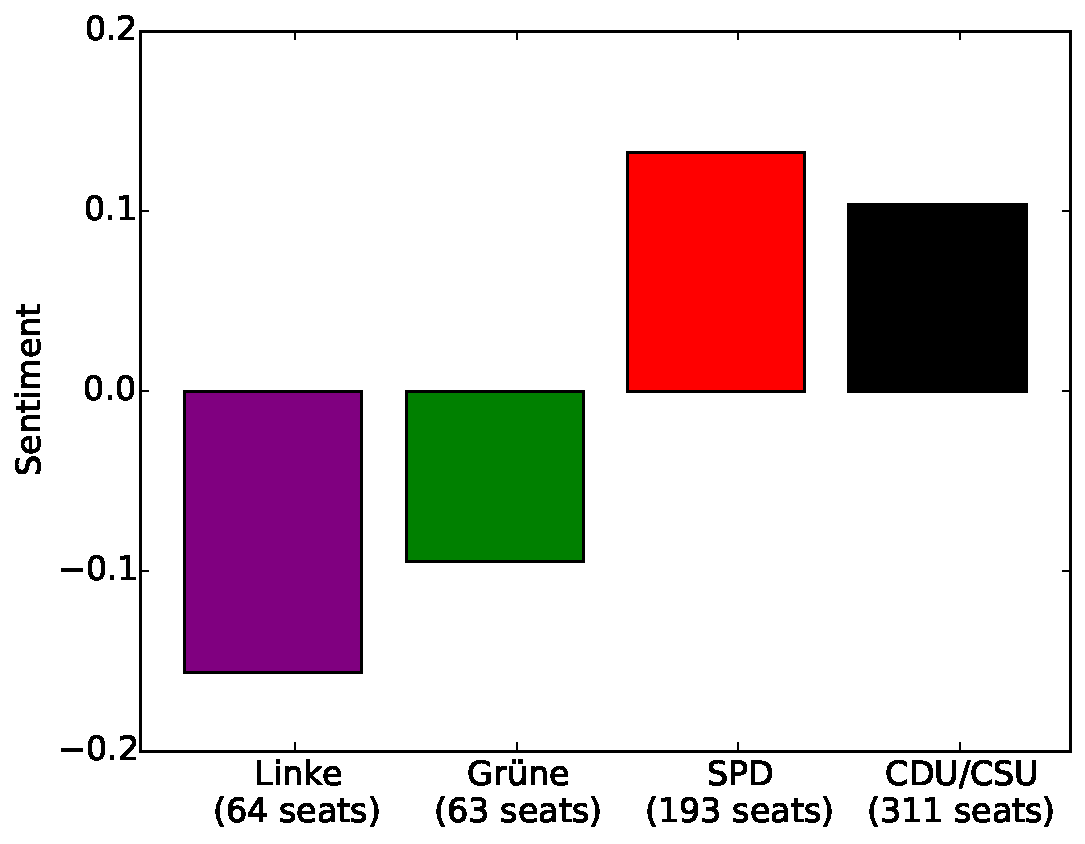
\includegraphics[width=8cm]{party_sentiments.pdf} 
%
\end{center}
\caption{
\label{fig:party_sentiments}
Speech sentiments computed for speeches of each party (parties are ordered according to political orientation from left to right). The more political power a party has (power is measured in seats in the parliament), the more positive the speech content is, the fewer seats a party has the more words associated with negative emotions are used in a speech.
}
\end{figure}

\section{Correlations between words and parties}\label{sec:word_party_correlations}

\autoref{fig:party_word_correlations} shows the correlations of individual words and each party. We plotted the top 20 words for each sign, i.e. the 20 words with the strongest positive and negative correlations for each party, respectively. While the correlations do indicate that there are -- despite extensive and careful cleaning procedures -- still words with strong correlations in the top words, we conjecture that at least some of these words do have some discriminatory power, even if they do not refer to political views. Below we list some examples, but the most prominent is probably: the opposition often addresses the government in their speeches, the govermental parties do that less often. This is reflected in the frequency of the usage of words that refer to members of the government or ministers. But among the often used and avoided words we also find words that refer to actual political content. Thus we hypothesize that to some extent these correlation coefficients can give hints as to what the bag-of-words histogram representation into which we transformed the speeches are related to the actual content of the speeches. In the following we give some examples of words that appear to be preferentially used or avoided by each respective party. Even though interpretations of these quantitative results are somewhat invalid, as they neglect the context in which these words were mentioned, we find some interesting patterns. 

\paragraph{Linke (left opposition)} The left wing opposition rarely mentions the daily agenda or interfraktional work; while the left opposition very often addresses the government and the ministers, as indicated by the words {\em Bundesregierung} (eng.: federal government), {\em Staatsminister} (engl.: federal minister), these addresses avoids the respectful introduction {\em verehrten}. Positively correlated words include {\em endlich} (engl.: finally), puts the focus on {\em Steuerzahler} (engl.: taxpayers), and {\em neoliberale} (engl.: neoliberal) attitudes that would promote {\em K\"urzungspolitik} (engl: cutting of investments in healthcare and social wellfare) while not being very sceptical towards ethically dubious economic practices, as alluded to by the words {\em Waffen} (engl.: Weapons) or {\em Profite} (engl,: profit) and {\em Profitinteressen} (engl: profit interests). Among the most often mentioned word in speeches of the left opposition is the word {\em Krieg} (engl.: war) -- the left opposition is often the first party to use this word and to advocate diplomatical alternatives, when other parties do not use this word at all and periphrase the same events with other words. 

\paragraph{G\"une (green/liberal opposition)}
Just like the left opposition also the more liberally minded green opposition very often addresses the federal government. The next-most likely words are however in contrast to the left opposition not words that refer to actual political content, but rather to words like {\em Nachfrage} (engl.: question) or {\em Zusatzfrage} (engl.: additional question), indicating that these formal steps to be taken by a party of the Bundestag to question certain political decisions of the government were indeed undertaken by the green party and that the party is talking about these inquirements. As to be expected from the political program of the green party, among the most often used words in their speeches include words related to ecological concerns, such as {\em Reaktorsicherheit} (engl.: security of nuclear plants), {\em Naturschutz} (engl.: environmental activities) and {\em Energie} (engl.: energy). 

\paragraph{SPD (social democrats)}
While we did filter out names of representatives in the parliament and of parties, some words that are part of a party name, like {\em Sozialdemorakte} (engl.: social democrats) are more general than the reference to that party only. As this word relates to political content, too, and in particular to the one represented by this party, it is often used in their speeches. the next most often used, interestingly, is {\em Koalitionsvertag} (engl.: contract of governmental coalition). The fact that the social democrats often use this word as often as their main political attitude could be interpreted as an often used argumentation strategy, in the sense of 'ok, we would love to do more socialdemocratic decisions, but we have to follow this contract, sorry'. In general the most often used words indicate a certain tendency for euphemistic formulations in the SPD, amongst the most often used words are {\em begr\"u\ss{}e} (engl.: to welcome), {\em freue} (engl.: being glad), {\em froh} (engl.: happy), {\em gut} (engl.: good). Rarely used words are among often related to the word {\em frage} (engl.: question), which can be interpreted as a more affirmative stance towards the work of the parliament. 

\paragraph{CDU/CSU (christian conservatives)}
While the oppositional parties have amongst their most often used words some that do refer to actual political content, the largest party in the government almost has almost exclusively words that relate to formal procedures in their top words list. An often used word is {\em Beschlussempfehlung} (engl.: recommendation for a decision), which refers to the work of commissions that give recommendations for political decisions, another often used word is {\em Tagesordnungspunk} (engl.: item on an agenda); also the focus is often put on previous {\em Vereinbarung[en]} (engl.: agreements) and {\em interfraktionell} (engl. between political parties) work. The less often used words include addresses to the governmental staff or words relating to questions. 

\begin{figure}
\begin{center}
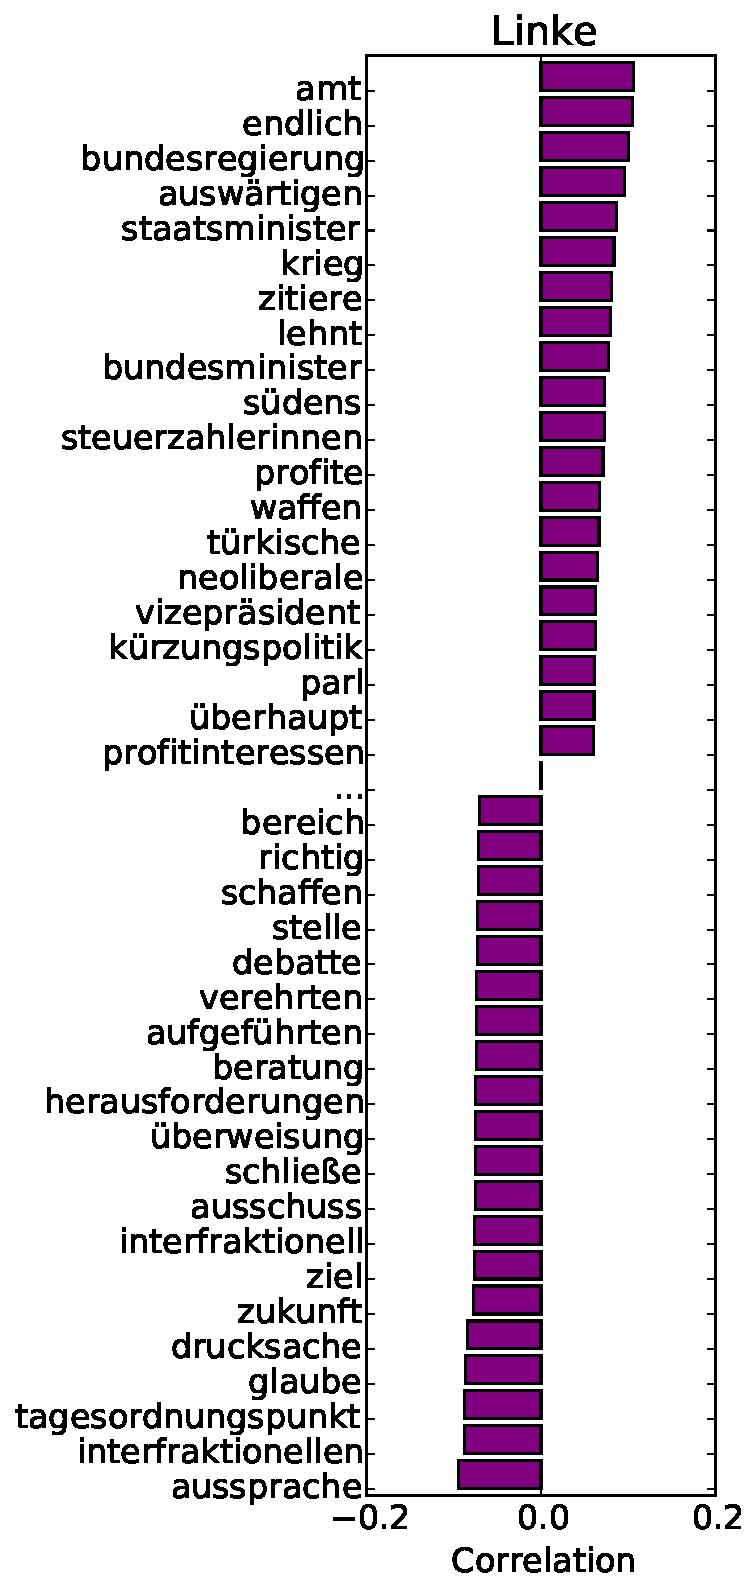
\includegraphics[width=3.5cm]{party_word_correlations-linke.pdf} 
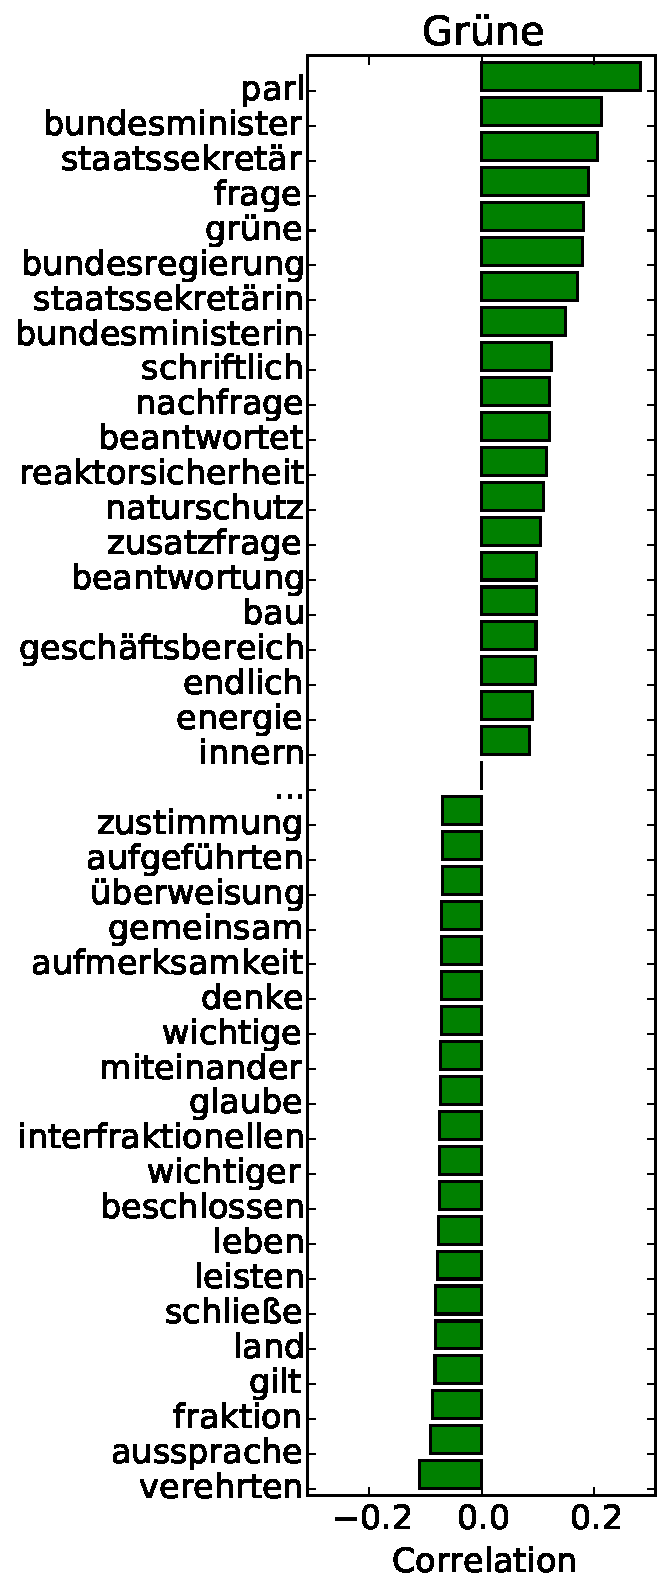
\includegraphics[width=3.1cm]{party_word_correlations-gruene.pdf} 
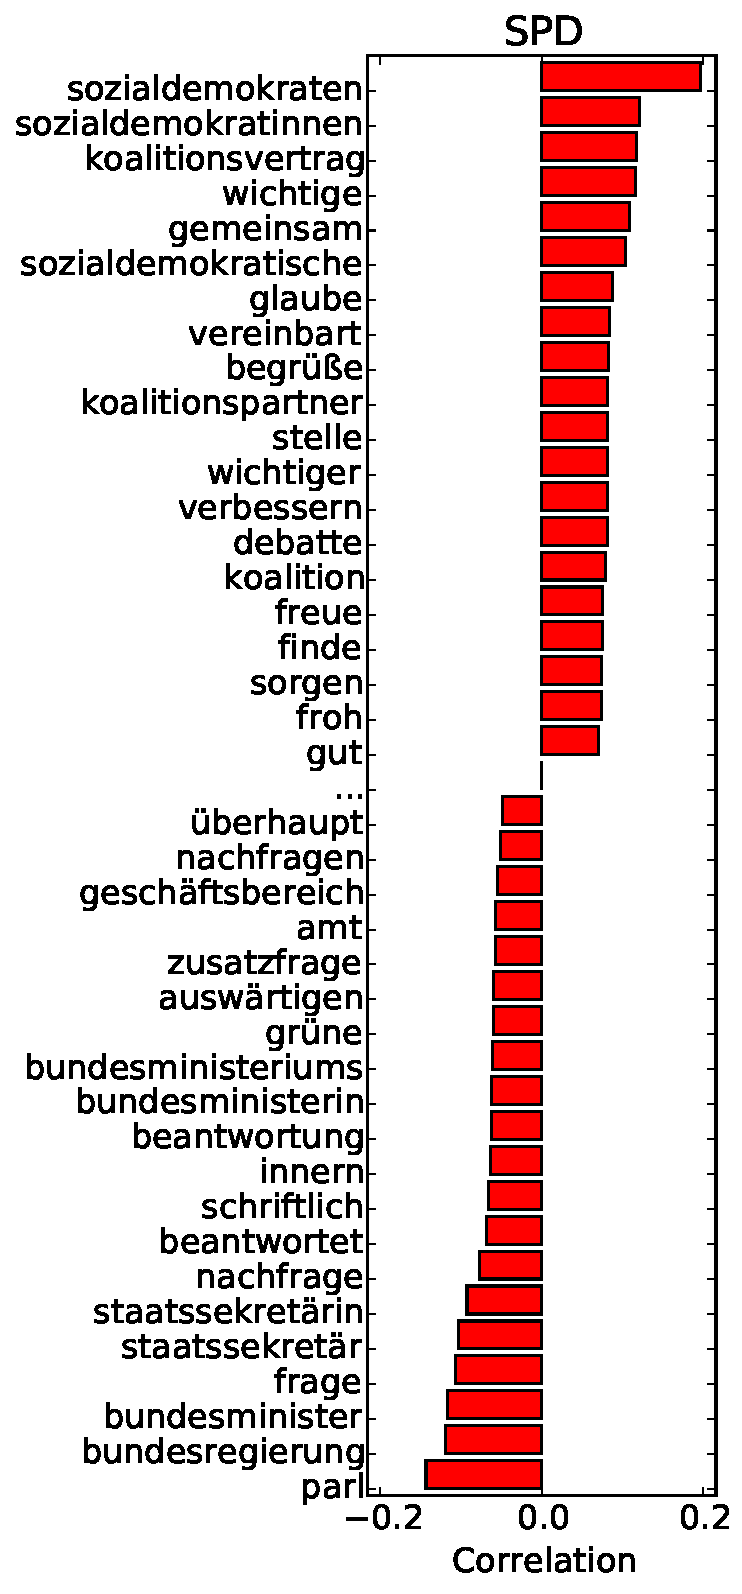
\includegraphics[width=3.45cm]{party_word_correlations-spd.pdf} 
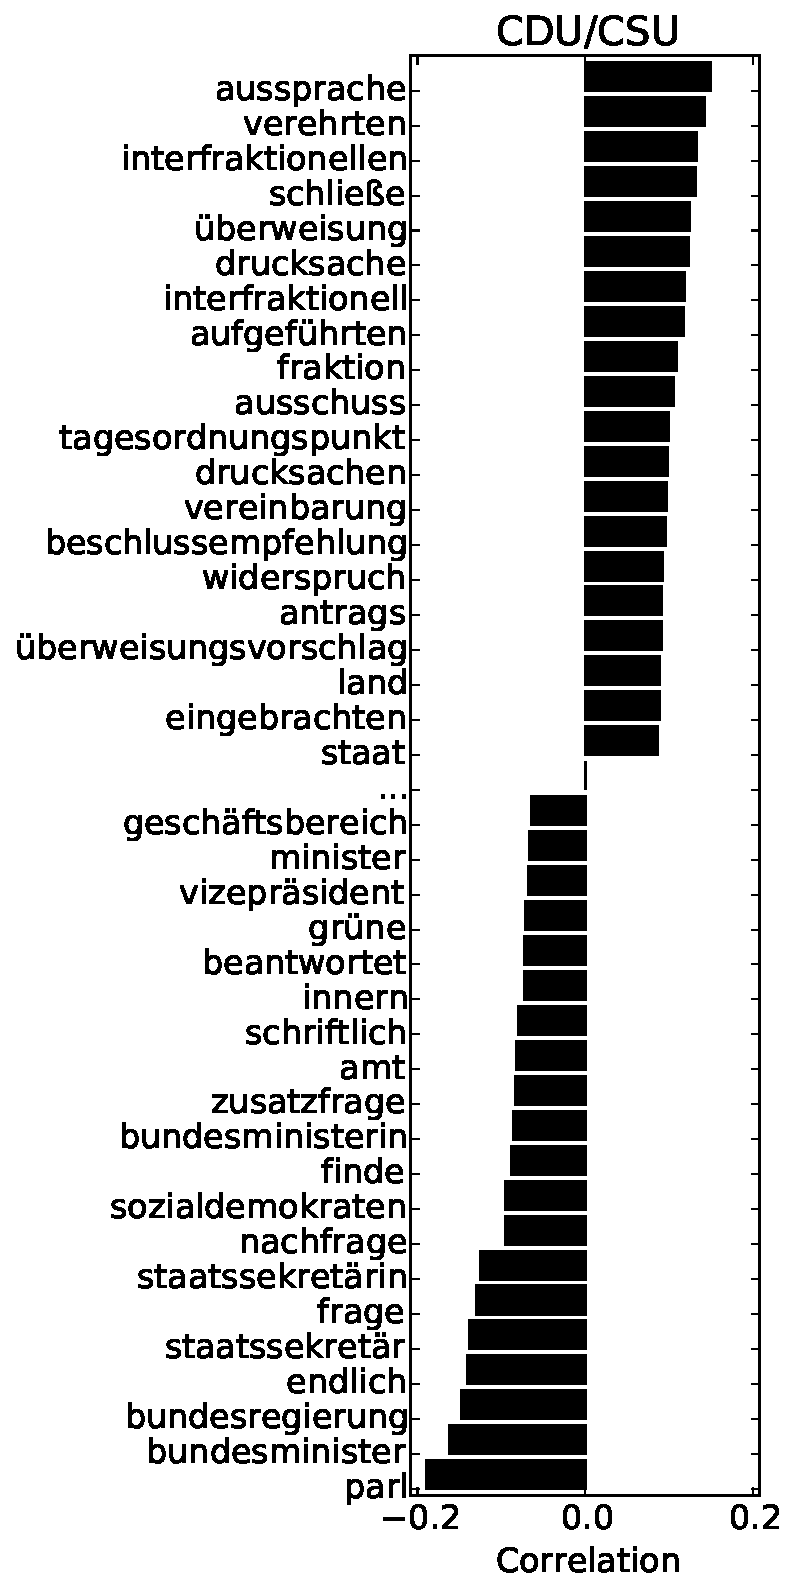
\includegraphics[width=3.65cm]{party_word_correlations-cdu.pdf}
%
\end{center}
\caption{
\label{fig:party_word_correlations}
Correlations between words and party for parliament speeches. }
\end{figure}

\section{Conclusion}
In this study we proposed a system that automatically associates texts with political parties. We performed extensive model selection on all parameters of the feature extraction as well as the model training and found that using rather simple methods we can obtain classification performances well above chance performance for both single party prediction as well as prediction of membership of the government or the opposition. While these results might not seem too surprising or useful, we emphasize that this is merely a first step, necessary 

\small{
\bibliographystyle{plain}
\bibliography{political_party_affiliation} 
}

\end{document}
